\section{Motivation}
%\begin{itemize}
%    \item Machine Hearing Principles
%    \item Spectrogram Based Machine Hearing
%    \item Case for Audio-Based Machine Hearing (w/ results teaser)
%\end{itemize}

We begin with an overview of machine hearing principles and make the case for 
an audio-centric CBAR technique.

\subsection{Machine Hearing Principles}
\label{motivation:machine-hearing}

Machine hearing is an emerging field focused on endowing machines with  
the ability to hear as humans do~\cite{lyon-human-2017}.
%However, this field has lagged behind computer vision due to its seeming lack
% of general applicability. 
%This is shown by the wealth of specialized music and
%speech sound analyses, with more general problems being ignored. 
The goal is to formulate a generalized model of sound with associated
representation, classification, and retrieval techniques. 
The architecture of an audio DBMS for machine hearning, that is inspired by the
human auditory system, consists of three components~\cite{lyon-machine-2010}:

\PP{Representation}
The first component, peripheral analyzer, is based on a part of the inner ear,
called \textit{cochlea} \footnote{Outer-ear structures are at the mercy of the
recording medium (\eg, the microphone).}. 
This spiral-shaped cavity is responsible for forming a representation of the 
given audio data.
by transforming acoustics into neural signals.
\textit{Reissner's membrane} is an important cochlear structure that can be
considered as a collection of band-pass filters, separating sounds into spectral
components~\cite{Plack2018}. These spectral components are then processed by
brain structures that convert the waveform representation to a more compact one.
 
The next step consists of creating an image representation of the given audio
data, thereby modeling the concept of human auditory sensory memory (\ie, echoic
memory) \AJ{Cite}.
The perception of sound depends on what comes before and occurs after an audio
segment. Thus, echoic memory determines human perception. 
It is critical in permitting the listener to integrate incoming information
with past events\footnote{Researchers have not reached consensus on the duration
of the memory  with estimates ranging from 250~ms to four
seconds~\cite{Wingfield2016}.}.
It is challenging to achieve high retrieval accuracy with only the image
representation and as such the next component is used for extracting key
features.

\PP{Classification}
The second component consists of feature extraction module that construct a more
compact and meaningful representation from the image formed by the previous
component.
This module most closely matches the \textit{neural code} of human audio
perception which forms the interface between sound and its conscious perception.
We note that the human auditory processing pipeline is still mostly unknown
and much of what we do know is speculative. 
It is hypothesized that multiple processes occur in
sequence to prepare the information for perception \cite{Eggermont2001}. 
It is likely these processing steps make actual perception less computationally
expensive. The output of this component determines the performance and
efficiency of the final component.

\PP{Retrieval}
This component takes in the representation formed by the previous module 
and maps it decisions. This component is analogous to conscious perception in
humans. It can vary from simple (\eg, a single perceptron) to complex
structures (\eg, a deep neural network).

\subsection{Image-Based Machine Hearing}
% \begin{itemize}
%     \item How this fits into Neural Coding and Echoic Memory
%     \item CNN approach
%     \item Autoencoding CNN approaches
%     \item Image retrieval (PAMIR approach)
% \end{itemize}

Given the high accuracy of content-based image retrieval (CBIR) systems, 
researchers have attempted to leverage these systems for audio retrieval.
Chechik et al. use a passive-aggressive model for image retrieval
(PAMIR) to perform audio retrieval over spectrogram imagery~\cite{Chechik2008}.
This technique consists of transforming audio recordings to spectrograms and
subsequently use image retrieval techniques for audio retrieval.
Thus, it leverages machine vision to perform machine hearing, thereby 
combining the neural coding and echoic memory portions of human hearing 
into a single step \footnote{The vision model is directly trained on
spectrograms instead of relying on a separate classification module.}.

%The PAMIR system uses probabilistic confidence to rank audio recordings based
% on their relevance to a text query.

\begin{figure}[!tbp]
    \centering
    \subfloat[Noisy]{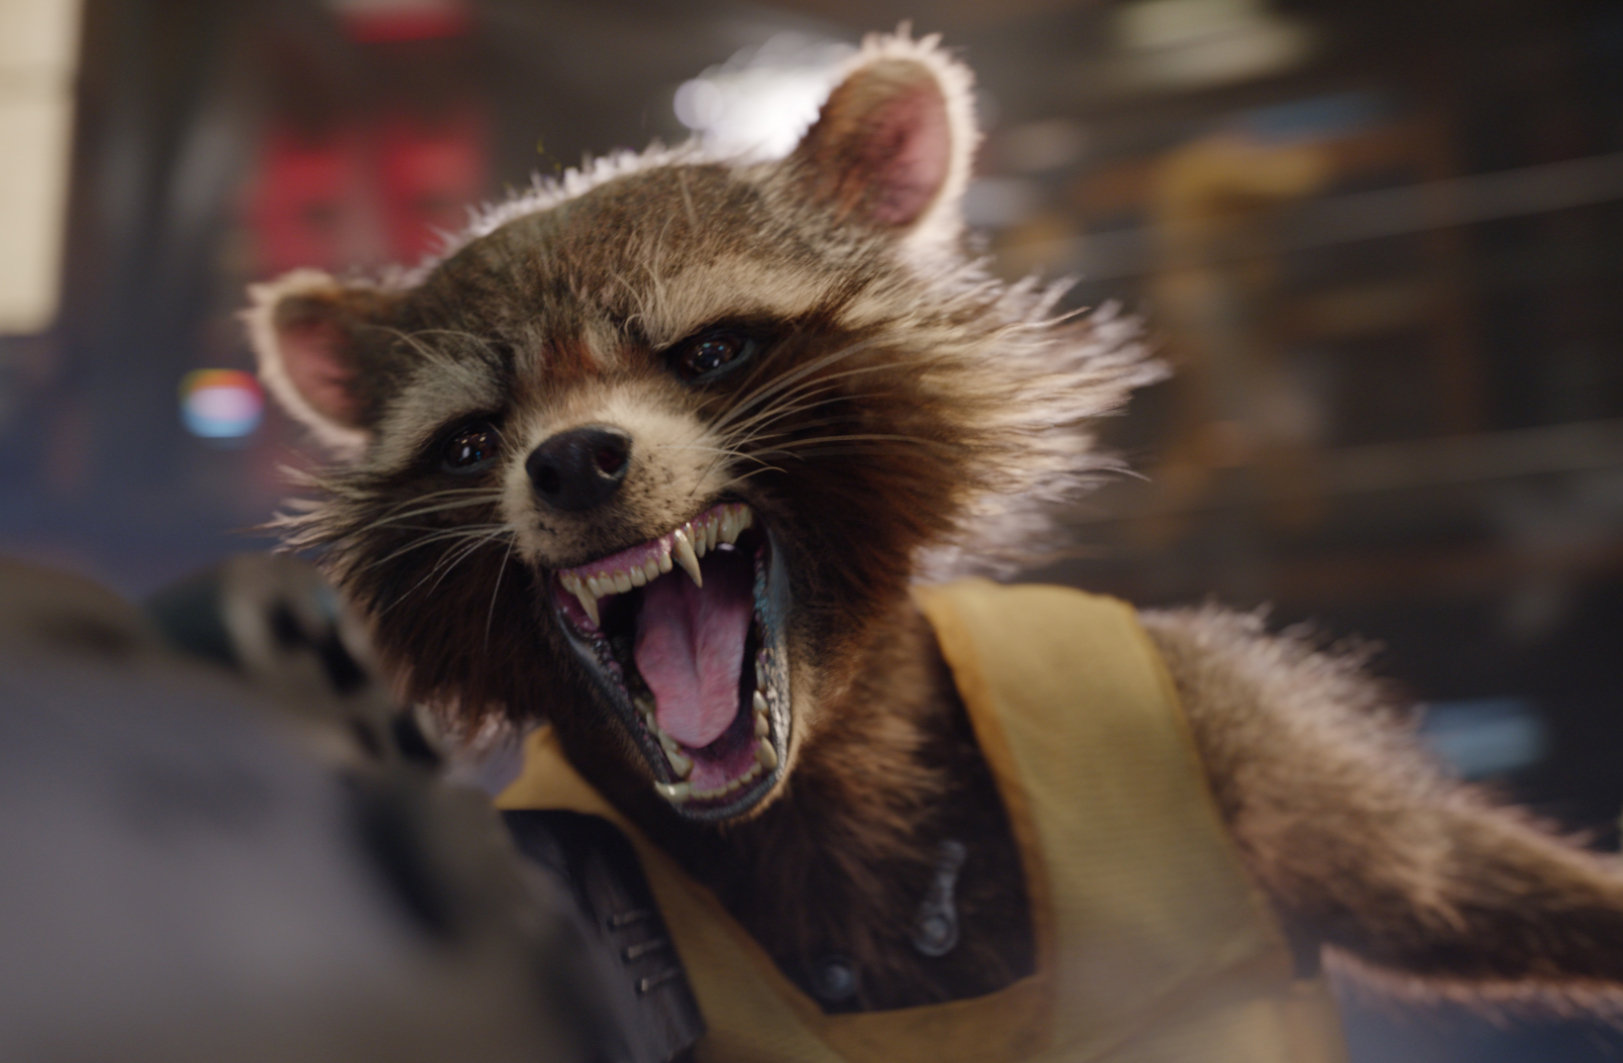
\includegraphics[width=0.5\textwidth]{figures/noisy-audio.jpg}\label{fig:noisy-audio}}
    \hfill
    \subfloat[Clean]{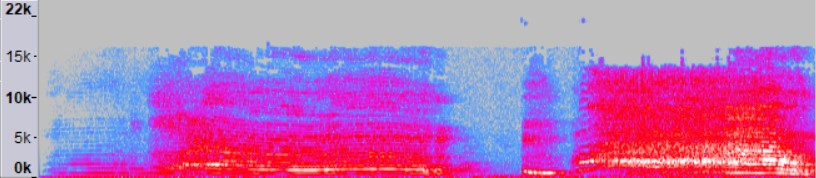
\includegraphics[width=0.5\textwidth]{figures/clean-audio.jpg}\label{fig:clean-audio}}
    \caption{Spectrograms illustrating the difference between clean and noisy audio when converted to the visual domain.}
    \label{fig:noisy-audio-cmpr}
\end{figure}

This approach for translating audio to a visual domain has seen some success,
especially in cases where audio events are isolated as illustrated
in~\cref{fig:noisy-audio-cmpr}.
However, in real-world audio recordings are typically generated from multiple
audio sources often with overlapping frequencies (\eg, group meetings).
This challenge stems from the \textit{transparency} of audio unlike images. 
Thus, a spectrogram is analogous to placing several transparent images 
over one another. 
State-of-the-art CBAR systems use a convolutional neural network (CNN) for 
image classification\AJ{Cite, describe CNN in a few sentences} and
train the CNN model on spectrograms.
However, these systems are unable to deliver high accuracy (> 70\%) even with
complex model ensembles~\cite{xu-large-scale-2018,piczak-environmental-2015}.

A more recent development in image-based machine hearing is to use an
unsupervised learning technique, called \textit{auto-encoding}\AJ{Cite?}. 
An auto-encoder is a type of neural network that learns to reconstruct its 
input image by reducing it to latent variables.
In image-based machine hearing, prior research has focused on reducing 
\textit{spectrogram}\AJ{define?} to latent variables using a CNN.
This approach suffers from the limitations discussed above.
While CNNs are effective on image recognition, they are unable to cope with the
transparency of audio. Furthermore, they ignore key features (\AJ{What?}),
thereby resulting in lower accuracy on real-world audio recordings with
multiple sources.

\subsection{Waveform-Based Machine Hearing}
% \begin{itemize}
%     \item Naive audio features
%     \item DTW + HMM
%     \item Autoencoding RNN approaches
%     \item Biologically Based Encoding
%     \item My approach + some teaser
% \end{itemize}

As an alternative to converting from an audio to visual domain, models can be trained on features from the audio itself. This approach to machine hearing hampers the ability of practitioners to apply proven image-based techniques but is overall more robust. In this approach, models are trained either directly on the audio waveform itself with no transformation, or a spectrogram is calculated and features are extracted from both the waveform and spectrogram.

With waveform-based machine hearing, \textit{Mel-frequency cepstral
coefficients} (MFCCs) are a frequently-used audio representation technique. 
The reasons for their popularity are twofold. First, they computationally
efficient to compute. Next, they provide a representation that is consistent
with human hearing~\cite{kaur-feature-2015}.
While certain audio processing tasks are feasible using only MFCCs, we require 
a more detailed representation for machine hearing\AJ{Cite?}.
A naive solution to this problem is to extract the temporal and spectral
features from the waveform to derive a more complete representation.
However, this approach is computationally expensive and leads to higher data
dimensionality resulting in slower convergence of classification agents.

Other techniques for constructing a detailed representation include: (1) 
Dynamic Time Warping (DTW) and (2) Hidden Markov Models (HMMs).
These approaches directly work on the audio data itself and thus do not require
feature extraction or constructions of spectral images.
They have found success in both speech recognition and specialized retrieval
systems\AJ{Cite?}.
Both DTW and HMMs have the benefit of taking referring back to previous states during determination, thus capturing the sequential nature 
of audio. 
However, DTW is computationally expensive and it is infeasible to support 
large audio databases using this technique.
Similarly, the complexity of HMMs increases when they need to support tens of
classes, as a model must be trained for each class.
Additionally, neither technique takes advantage of domain knowledge 
and do not conform to the machine hearing principles outlined
in~\autoref{motivation:machine-hearing}.

While auto-encoding with CNNs does not work well for audio retrieval,
encoders based on Recurrent neural network (RNN) do not suffer from this
limitation.
This is because much of the information in a audio recording is dependent 
on what comes before it.
Unlike CNN-based encoders that learn from the spectrogram image,
RNN-based encoders learn from the waveform values or vectors of spectrogram
features presented as a time series.
The latter approach has two additional benefits.
First, RNN-based encoders are computationally efficient.
Second, they create compact representations that take time into account 
and can be used with any number of off-the-shelf classifiers.

\AJ{Why do we need the following paragraph? --
Researchers continue to seek the biological neural code for audio
encoding~\cite{Eggermont2001}. 
Through studies of the biological systems that convert sound waves to neural
responses, researchers have been able to emulate certain steps of the audio
encoding pipeline with other steps requiring speculation. 
Smith and Lewicki present a non-linear model based on population spike code 
to encode waveforms~\cite{smith-efficient-2006}. 
They illustrate that idealized spikes encode precise temporal positions and
magnitudes of underlying acoustic features. 
This effort provides a method to efficiently extract a coding of natural 
sounds, making sure the classifiers are working with an information-rich
representation.
}

\begin{table}[t]
    \centering
    \begin{tabular}{cccccc}
                & Bag of Features & DTW & HMM & Wavelet  \\ \hline
    Approx Size & a & a & a & a \\
    Complexity  & a & a & a & a
    \end{tabular}
    \caption{Simple table with audio representations and their complexity/usefulness/features}
    \label{tab:audioreps}
\end{table}

We next describe the three components of \sys in detail.
